% --------------------------------------------
%		CAPITOLO 5
%---------------------------------------------

\chapter{TJ-Monopix 2 characterization ??}
%\addcontentsline{toc}{chapter}{Caratterizzazione di TJ-Monopix 2}

\section{Matrix and flavors}

\subsection{Mask (operation) and noisy pixels}

\subsection{Analog and digital readout}

\subsubsection{BCID reset}
\begin{comment}
REFERENZE
\end{comment}

\subsubsection{Main registers (and conversion?)}



\subsection{Comparison between data and simulation}
%\addcontentsline{toc}{subsection}{Confronto degli andamenti con le simulazioni}

In the interest of understanding how the settings of the chip influence the threshold's value, several measurements have been taken varying the values of the main registers which are responsible for it.
The results are compared with simulations done by Hung Pham (...). [???]

\subsubsection{$I_{CASN}$}

This current is responsible of the output baseline. In a few words, higher this value, higher the baseline, lower the threshold and also a little bit the gain.

In figure \vref{fig:icasn_sim}, we can see the simulated behaviour of the threshold and the gain, increasing the value o $I_{CASN}$.

\begin{figure}[h!]
\centering
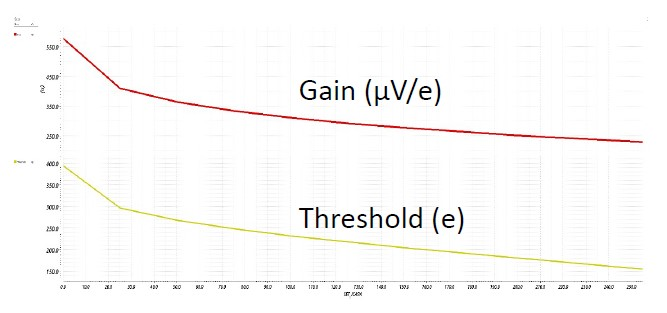
\includegraphics[scale=.9]{thr_gain_icasn(sim)}
\caption{Trends of Gain and Threshold increasing $I_{CASN}$.}
\label{fig:icasn_sim}
\end{figure}

To verify the trend of threshold in particular, three different acquisition have been taken by fixing $I_{THR}$ = 20, 40, 64 and increasing $I_{CASN}$ from 0  to 30 DAC, with a step of 5 DAC. We have done this enabling 200 pixels in the Cascode FE (rows: 472 - 512, cols: 225 - 230).[??]\\

The threshold distributions have been fitted with a gaussian function for each measurement,  in order to obtain the average values and their dispersion.

\begin{itemize}
\item[$I_{THR}=64$]:

\begin{tabular}{c | c | c}
$I_{CASN}$ [DAC] & THR [DAC] & THR Dispersion [DAC]\\
\hline
0 & 61.43 & 2.45\\
5 & 53.42 & 2.45\\
10 & 50.33 & 2.45\\
15 & 48.21 & 2.41\\
20 & 46.70 & 2.38\\
25 & 45.49 & 2.52\\
30 & 46.09 & 2.50
\end{tabular}

\item[$I_{THR}=40$]:

\begin{tabular}{c | c | c}
$I_{CASN}$ [DAC] & THR [DAC] & THR Dispersion [DAC]\\
\hline
0 & 47.28 & 2.12\\
5 & 41.07 & 2.02\\
10 & 38.39 & 2.03\\
15 & 36.65 & 1.95\\
20 & 35.53 & 1.91\\
25 & NaN & NaN\\
30 & 33.37 & 2.04
\end{tabular}

[Here we can see a particular setting, that is $I_{THR}=40$ AND $I_{CASN}$=25, for which the chip doesn't seem to work.
PIXEL THAT FIRE UP??]

\item[$I_{THR}=20$]:

\begin{tabular}{c | c | c}
$I_{CASN}$ [DAC] & THR [DAC] & THR Dispersion [DAC]\\
\hline
0 & 34.43 & 1.95\\
5 & 28.10& 1.72\\
10 & 26.59 & 1.75\\
15 & 24.66 & 1.77\\
\end{tabular}
\medskip\\

\end{itemize}

In figure \vref{fig:alltrends_icasn} all trends obtained from these data are reported.

[TREND OF DISPERSION?]

\begin{figure}[h!]
\centering
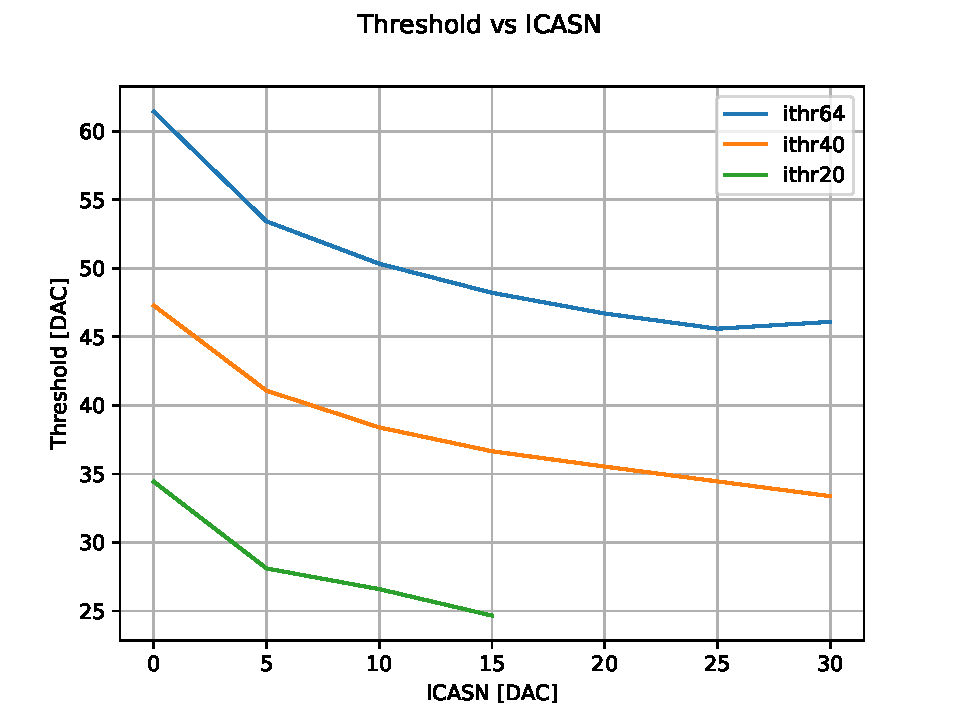
\includegraphics[scale=.7]{all_trends(ICASN)}
\caption{Threshold vs. $I_{CASN}$ for $I_{THR}$= 20, 40, 64.}
\label{fig:alltrends_icasn}
\end{figure}

\subsubsection{$I_{THR}$}

Reusing the same data of the previous measurements, the trend of the threshold have been studied, changing the value of $I_{THR}$ and fixing that of $I_{CASN}$. In this case only $I_{CASN}$ from 0 to 15 DAC is considered, because for higher values we don't have enough measures of the threshold (specifically only two for $I_{THR}$=40, 64). The results are shown in figure \vref{fig:alltrends_ithr}.

\begin{figure}[h!]
\centering
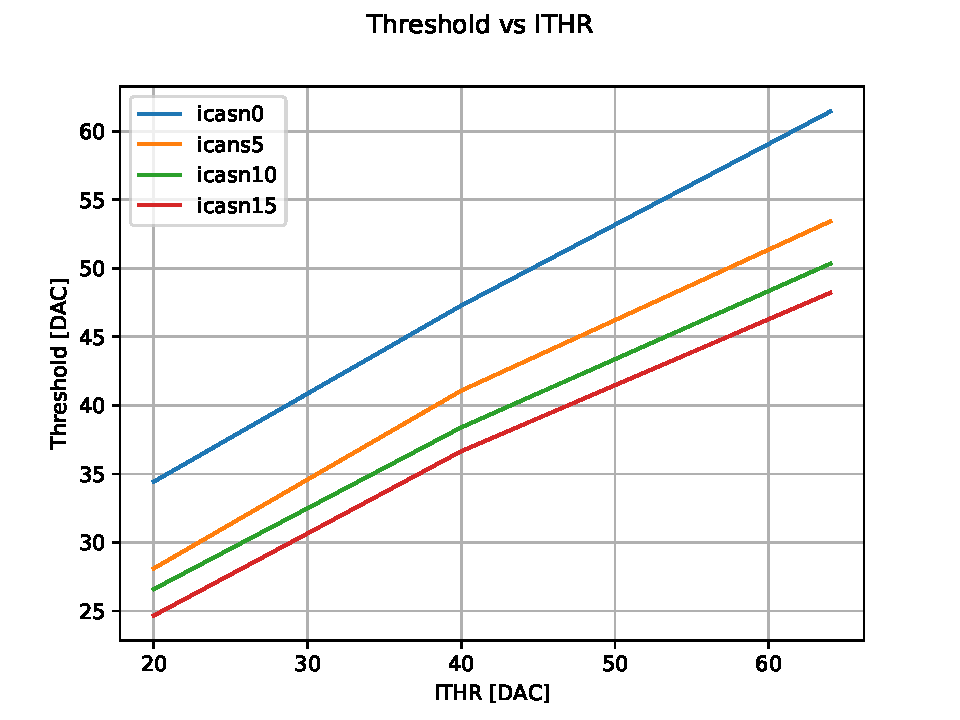
\includegraphics[scale=.7]{all_trends(ITHR)}
\caption{Threshold vs. $I_{THR}$ for $I_{CASN}$= 0, 5, 10, 15.}
\label{fig:alltrends_ithr}
\end{figure}

We can compare them with the simulation done by Hung Pham in figure \vref{fig:ithr_sim}. 

\begin{figure}[h!]
\centering
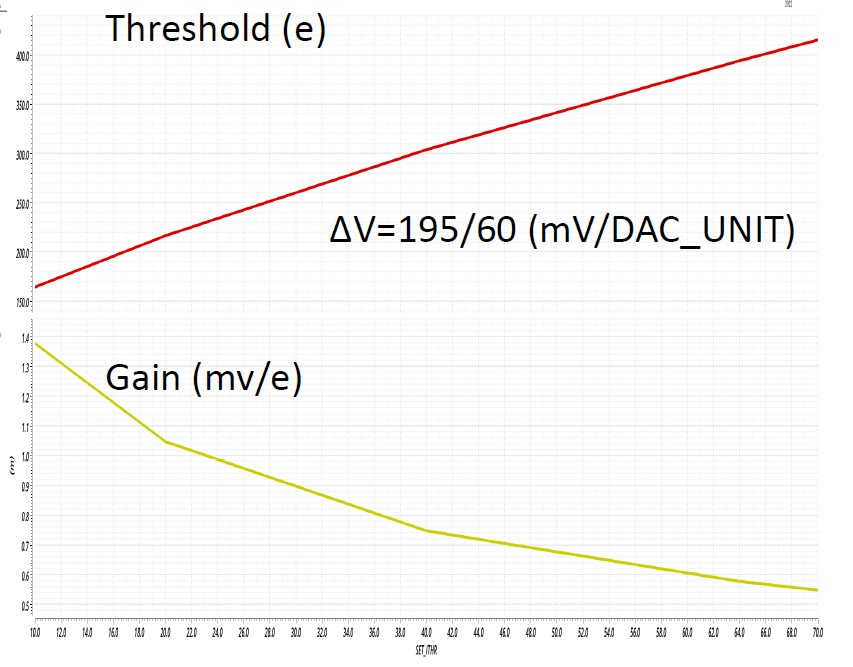
\includegraphics[scale=.7]{ithr_simulation}
\caption{Trends of Gain and Threshold increasing $I_{CASN}$.}
\label{fig:ithr_sim}
\end{figure}

\subsubsection{$V_{CASP}$}

[Explain VCASP]

In order to enhance this type of analysis, other scans have been run increasing the value of $V_{CASP}$ from 3 to 143, with a step of 10 DAC unit. In figure \vref{fig:th_vs_casp} the threshold's trend with respect to different values of this register.

\begin{figure}[h!]
\centering
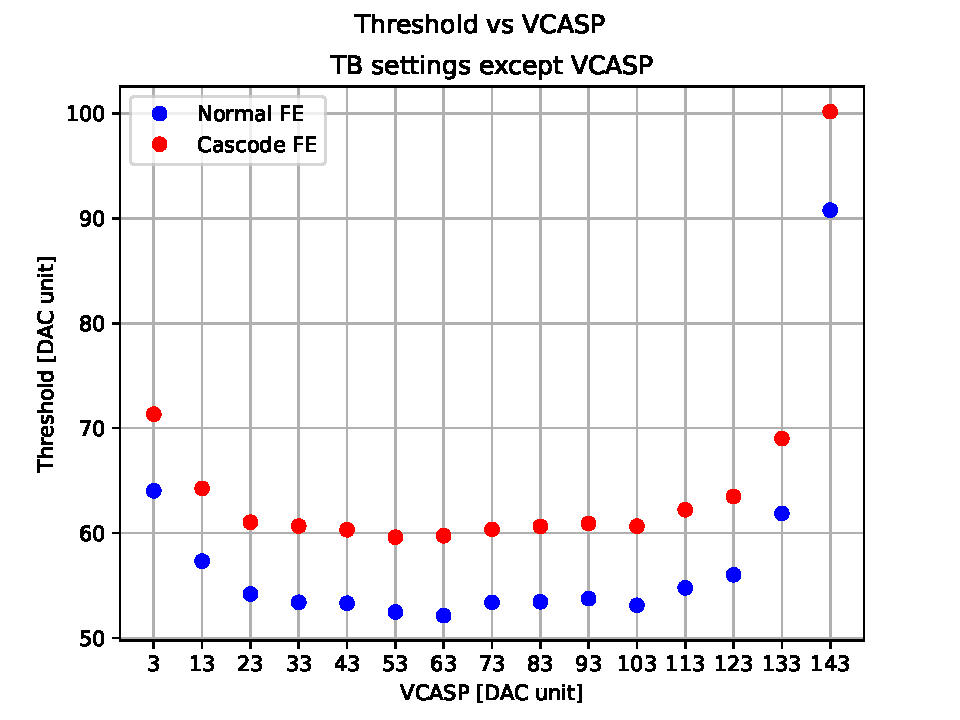
\includegraphics[scale=.7]{TH_vs_VCASP(point)}
\caption{Trends of Threshold increasing $V_{CASP}$.}
\label{fig:th_vs_casp}
\end{figure}



\subsubsection{Time over Threshold (ToT)}

The last analysis done in order to make a comparison with the simulations, is about the trend of the ToT changing the value of $I_{CASN}$ for a fixed value of $I_{THR}$ and vice versa. In particular we consider the data obtained with $I_{CASN}$ fixed to 0 DAC and $I_{THR}$ to 64 DAC, which are the values studied and used for this registers during the Test Beam in Desy.

\begin{figure}[h!]
\centering
\subfigure[ToT vs $I_{THR}$ ($I_{CASN}$=0 DAC) - Data (\textbf{Cascode})]
{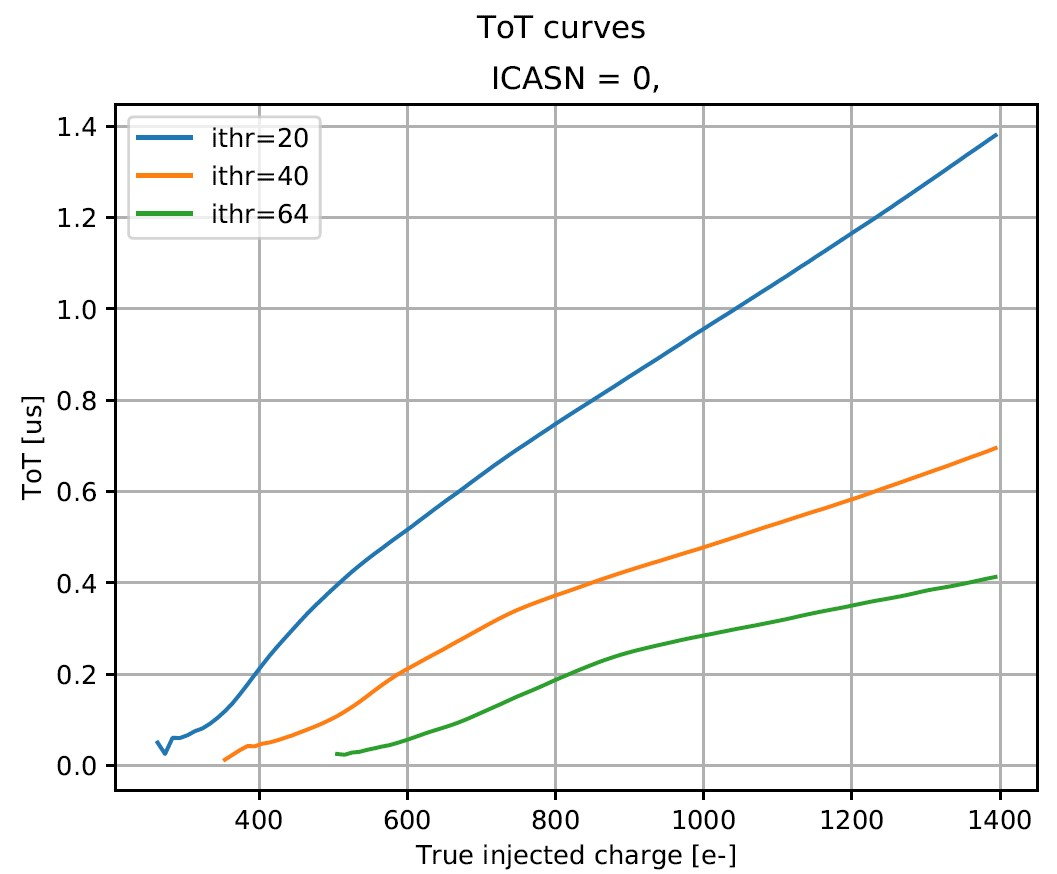
\includegraphics[scale=0.5]{tot_curves_icasn0}}\quad
\subfigure[ToT vs $I_{THR}$ ($I_{CASN}$=0 DAC) - Simulation]
{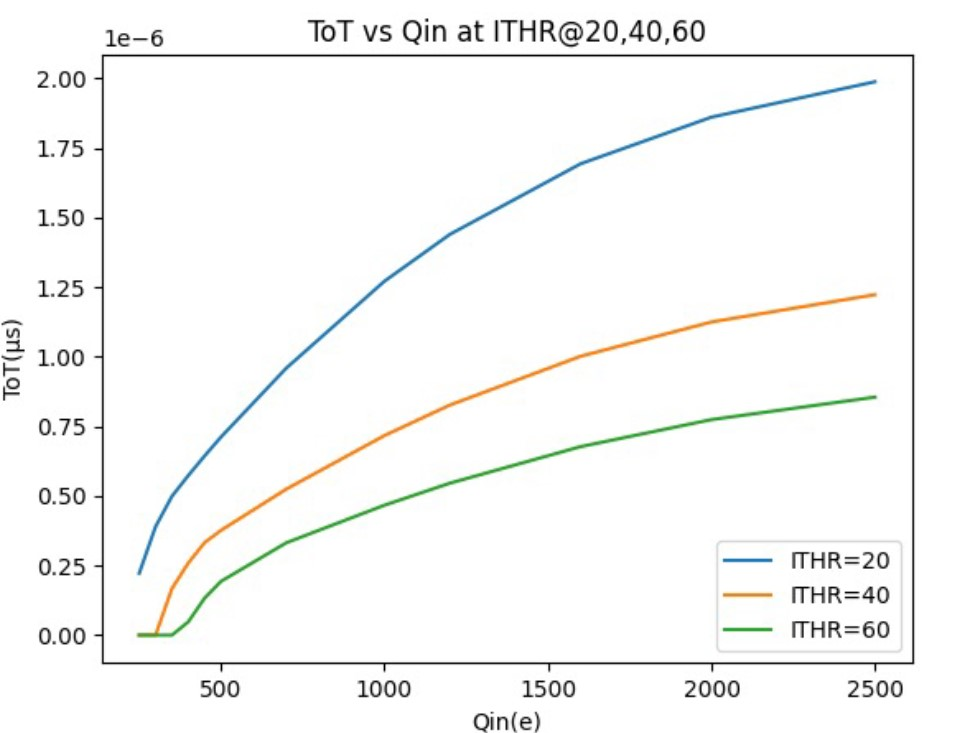
\includegraphics[scale=0.4]{tot_curves_icasn0_simu}}\\
\caption{ToT vs $I_{THR}$}
\label{fig:tot_vs_ithr}
\end{figure}

\begin{figure}[h!]
\centering
\subfigure[ToT vs $I_{CASN}$ ($I_{THR}$=64 DAC) - Data (\textbf{Cascode})]
{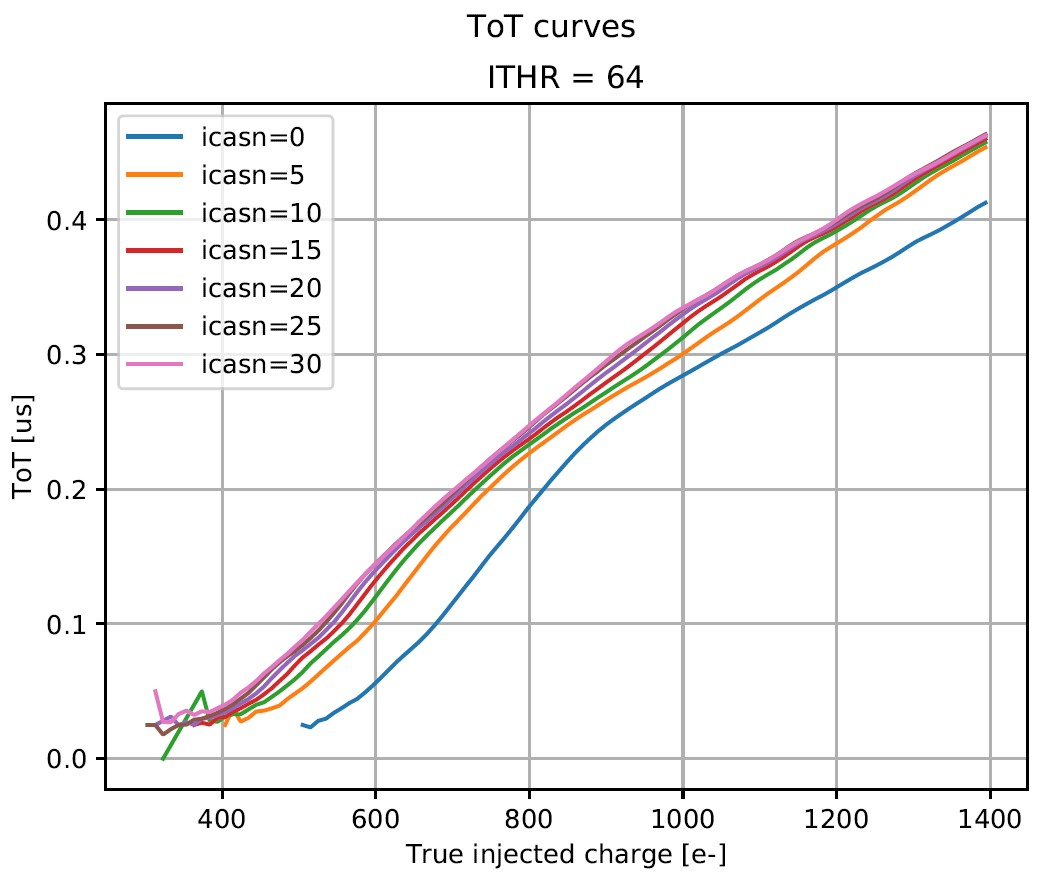
\includegraphics[scale=0.5]{tot_curves_ithr64}}\\%\quad
\subfigure[ToT vs $I_{CASN}$ ($I_{THR}$=64 DAC) - Simulation]
{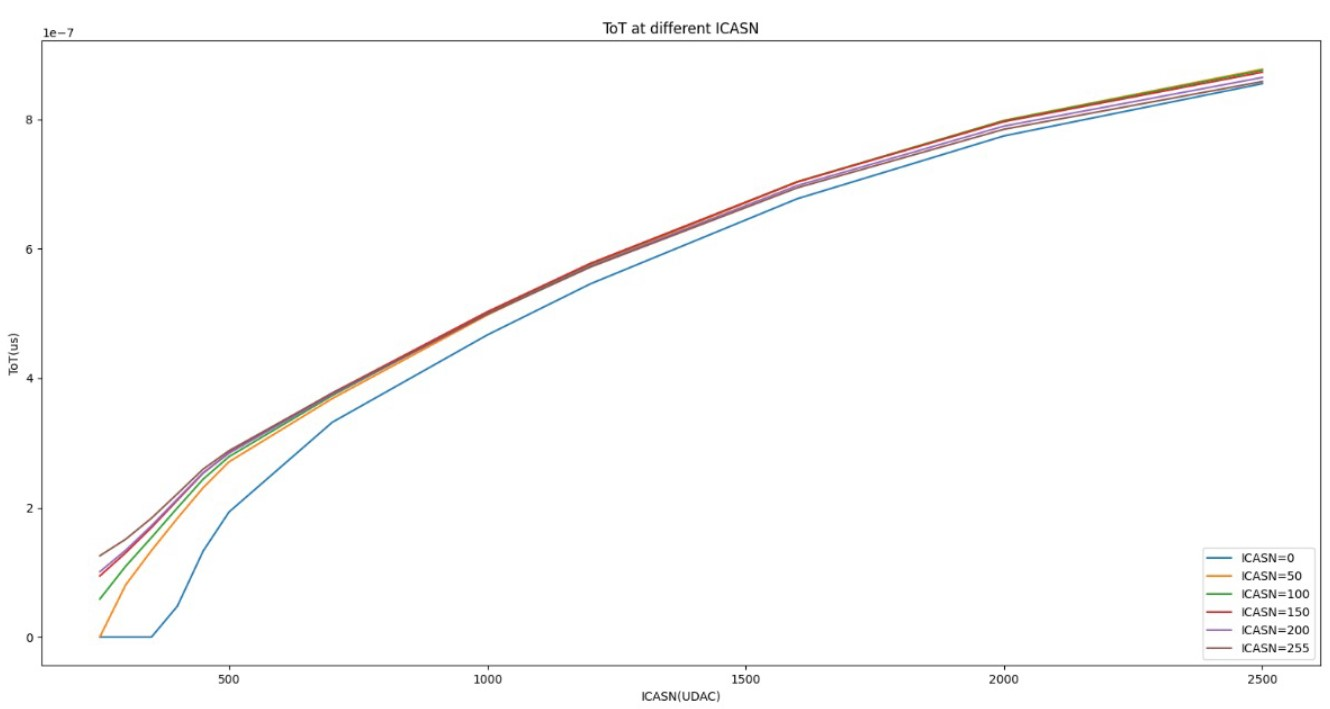
\includegraphics[scale=0.35]{tot_curves_ithr64_simu}}\\
\caption{ToT vs $I_{CASN}$}
\label{fig:tot_vs_icasn}
\end{figure}


In the last plots of this section (\vpageref{fig:tot_vs_vcasp}) are reported the trends of the ToT varying the value of $V_{CASP}$ for both Normal and Cascode FE, but there aren't simulations to make a comparison. 

\begin{figure}[h!]
\centering
\subfigure[ToT vs $V_{CASP}$ - Data (\textbf{Cascode})]
{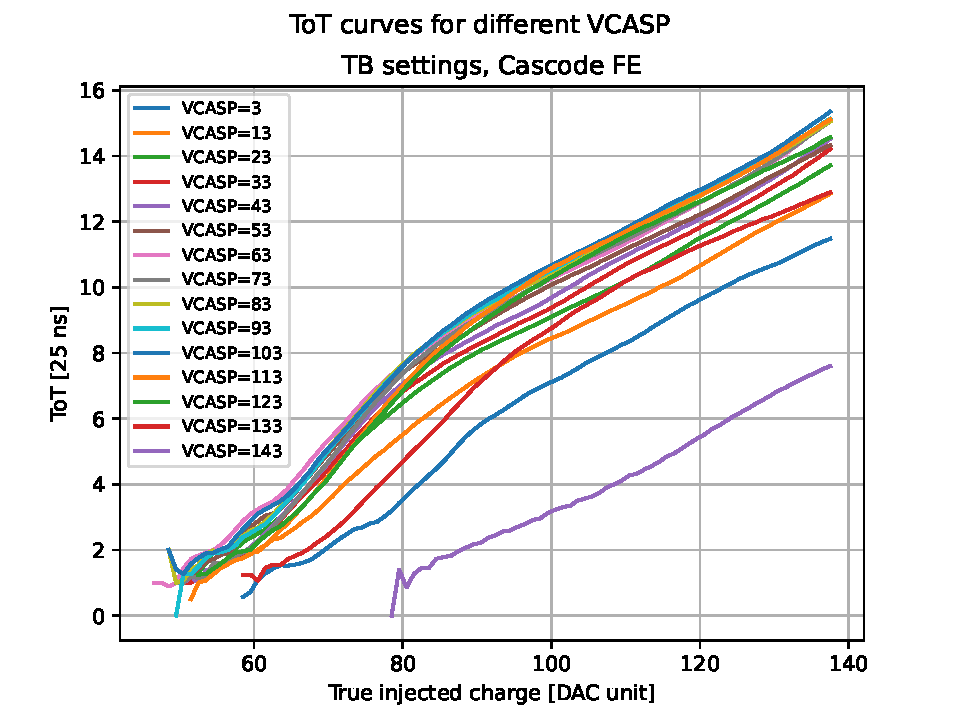
\includegraphics[scale=0.4]{tot_vcasp(cascode)}}\quad
\subfigure[ToT vs $V_{CASP}$ - Data (\textbf{Normal})]
{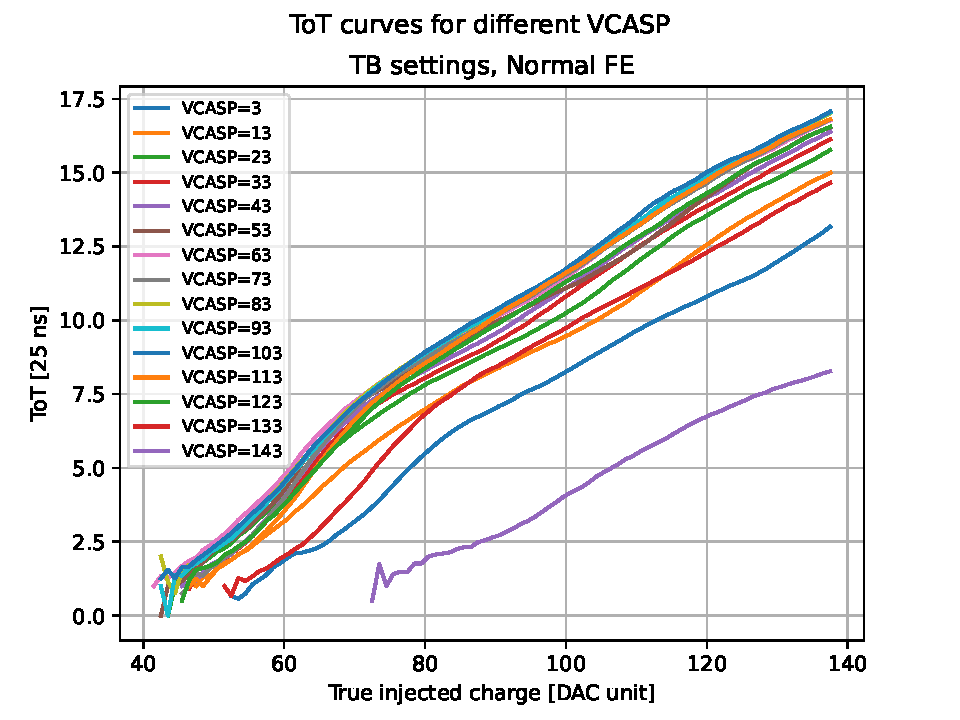
\includegraphics[scale=0.4]{tot_vcasp(normal)}}\\
\caption{ToT vs $V_{CASP}$}
\label{fig:tot_vs_vcasp}
\end{figure}



\section{Characterization by injection}
%\addcontentsline{toc}{section}{Caratterizzazione tramite l'iniezione}

The ultimate purpose of this measurement is to describe (characterize) the response of each pixel by injecting a charge equivalent to the typical energy released from particles emitted in decays of radioactive materials. As explained in the previous section (reference), for example the \ch{^{55}Fe} has an emission spectrum with quite sharp lines and this allows to compare data more easily. The first line is at 5.9 KeV which corresponds on average to about 1616 $e^{-}$ released (through the pixel??).
For this reason it's mandatory to know the conversion between DAC and $e^{-}$ [reference?] and to inject charges in order to study the pixel behaviour in the right regions, so those which are more interesting from a physical point of view.

Preliminarly it was necessary to study the threshold distribution on the whole matrix. The four flavors have been separately analyzed to be able to study their main difference concerning their performance and features.

\begin{figure}[h!]
\centering
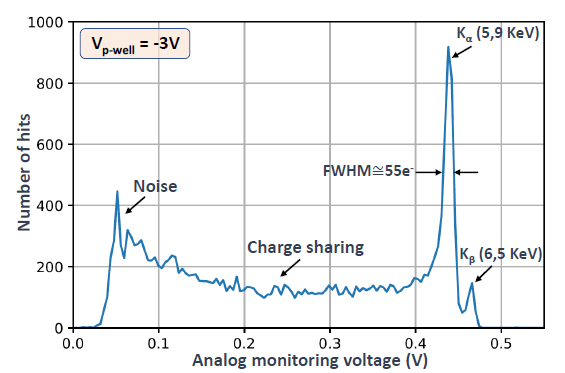
\includegraphics[scale=0.8]{spectrum_fe}
\caption{\ch{^{55}Fe} (radiactive source) emission spectrum using the analog output of a PMOS reset front-end of TJ-Monopix 1. (reference)}
\label{fig:fespectrum}
\end{figure}

%------------------------------------------------------------
\subsection{Injection circuit issues}

In carrying out the measurements mentioned above, we started to noticed some issues with the injection circuit, which seemed to limit its working range. As a matter of fact the height of the injection pulse is expected to grow linearly increasing the value of charge to be injected.
It actually happened up to a value of (about) $\approx$ 140 DAC, but for higher quantities of injected charge, the circuit seemed to increase not only the height of the signal, but also the threshold by a certain amount of $\Delta V$ (or equivalently of $\Delta Q$, related by the conversion factor reported in REFERENCE). Moreover, for injection height grater than 200 DAC, only the threshold grows, without increasing the actual injected charge in any way.\\
We come to the conclusion that the grows of the threshold was artificial and due to the failure of the injection circuit.[?]

However as we have seen in the previous section (reference), the threshold depends on the settings of the chip registers and it can't be influenced by the injected charge, otherwise the whole response of the chip would be chaotic and it would not be reliable to take precise measurement of the impinging particles. 

For this problem, the investigation on the behaviour of the threshold and its dispersion of all flavours of the matrix, required a series of additional measurements.\\
In the following sections the method used to obtain a reliable value of threshold and ToT is explained.

%-------------------------------------------------------
\subsection{Measurement of the average threshold shift for injected charge greater than 140 DAC}

To evaluate this artificial shift of the threshold, two different measurements have been done for each flavor:

\begin{itemize}
\item for an injected charge equal to 140 DAC $\rightarrow$ before the saturation region;
\item for an injected charge equal to 200 DAC $\rightarrow$ almost the maximum limit of the saturation region (from this value onward only the threshold increases, not the injected charge).
\end{itemize}

The threshold distributions obtained from each measurements have been fitted to extract an average value on the whole flavor. Naming $Q_{th, 140}$ and $Q_{th, 200}$  the threshold obtained from injections of 140 and 200 DAC respectively, the mean shift has been estimated by:

\begin{equation}
\Delta Q = Q_{th,200} - Q_{th,140}
\end{equation}

Eventually, this charge shift has been subtracted from data collected for an injection pulses of 200 DAC, in order to extrapolate the response in ToT of the injected pixels up to a value of 170 DAC.

What has been obtained is reported in the following section, together with a briefly explanation of the method used to evaluate the threshold.


%--------------------------------------------------------------------
\subsection{Threshold and S-Curve}
%\addcontentsline{toc}{subsection}{Curva S e threshold}

In order to obtain the thresold value for all pixels, each one of them has to be injected an arbitrary number of times (100 times in this work) for each value of the injection pulse between a minimum value, chosen setting the chip register ''\textbf{VL}'' and a maximum value set by the ''\textbf{VH}'' register, with a step of 1 DAC unit this is also adjustable).

So for each injection pulse height, the mean of 100 injection output are considered. In this way plotting the average number of detected hits in function of the injected charge, the typical curve better known as ''\textit{S-curve}'' is reconstructed. It can be fit with the \textit{error-function},
\begin{equation}
error func
\end{equation}
 
from which the value of the threshold is evaluated considering the value of the injected charge at half of the curve's maximum height.

Specifically plotting the number of hits observed on each pixel divided by the total number of injections, for each injected charge, the half height corresponds to a charge value for which the pixel detects 50 hits of 100 injected and so when it has an occupancy of 0.5.

%%%%SPIEGARE METODO DI LUDOVICO???? 


%%%METTI ESEMPIO S-CURVE
\begin{comment}
\begin{figure}
\centering
\includegraphics[]{}
\caption{An example of the S-Curve and the evluation of the threshold.}
\label{ex_scurve}
\end{figure}
\end{comment}

In the following are reported the results of this study for the flavors of all matrix.

\subsubsection{Normal FE}

The first flavor of the matrix is the \textbf{Normal FE}, which consist of 512 rows and 224 columns for a total of 114.688 pixels. In figure \vref{fig:norm_scurve_140} are plotted all the s-curves of the all well-functioning Normal flavor pixels. The chip registers have been set with the same values used during the Test Beam at Desy (during...) which are reported in table \vref{tab:tb_settings}.

\begin{table}[h!]
\centering
\begin{tabular}{>{\columncolor{BrickRed}} c|c}
\rowcolor{lightgray}
Registri & Default Settings (''GOE'') \\
\hline
ITHR & 64 \\
\hline
IBIAS & 50 \\
\hline
VRESET & 143 \\
\hline
ICASN & 0 \\
\hline
VCASP & 93 \\
\hline
VCASC & 228 \\
\hline
IDB & 100 \\
\hline
ITUNE & 53 \\
\hline
VCLIP & 255 \\
\hline
ICOMP & 80 \\
\hline
IDEL & 88 \\
\hline
IRAM & 50 \\
\hline
\end{tabular}
\caption{Settings of the main registers used for the W14R12 chip, for Normal and Cascode flavors, during the Test Beam in Desy.}
\label{tab:tb_settings}
\end{table}

\begin{figure}[h!]
\centering
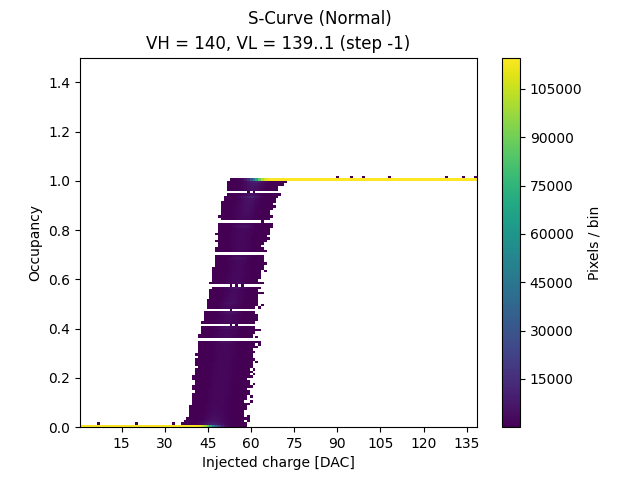
\includegraphics[scale=.6]{all_norm_thscan_140}
\caption{S-curves of all pixels of the Normal FE with an injection pulse of 140 DAC.}
\label{fig:norm_scurve_140}
\end{figure}

Using this setting, none of the pixels were noisy and so it wasn't necessary to use any mask.

As already explained (in section...) the threshold distributions obtained from the two different measurements with an injection pulse of 140 and 200 DAC respectively, have been fitted and they are shown in figure \pageref{fig:thdist_norm} as representative examples also for the others flavors.

\begin{figure}[h!]
\centering
\subfigure[VH = 140 DAC]
{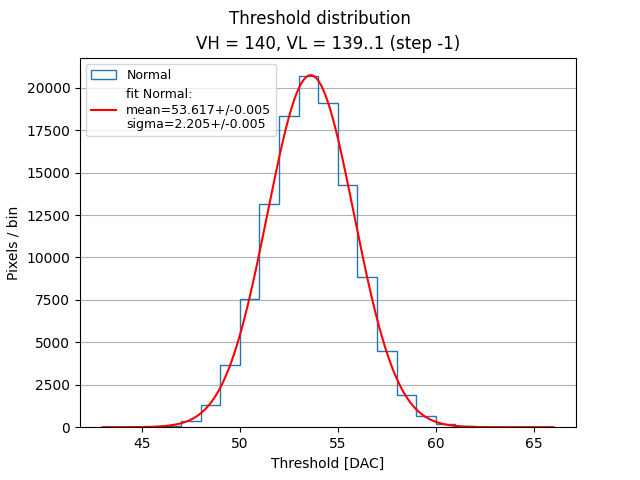
\includegraphics[scale=0.6]{all_norm_thdist_140}}\quad
\subfigure[VH = 200 DAC]
{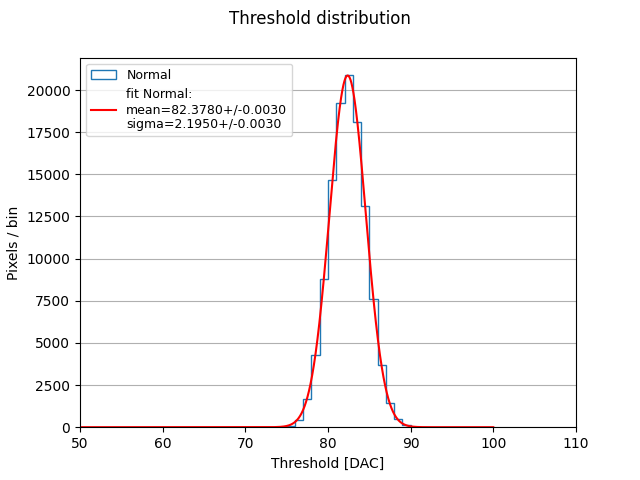
\includegraphics[scale=0.6]{all_norm_thdist_200}}\\
\caption{Threshold distributions of \textbf{Normal} flavor before and at the maximum saturation, respectively.}
\label{fig:thdist_norm}
\end{figure}
 
\begin{comment}
For the greater (higher) injection height, 8 different measurement have be actually done, each one on 28 consecutive columns and on all rows. Then data have been put together to obtain a single (summary) plot on the whole flavor. Same procedure has been preformed on the \textbf{Cascode FE}.
\end{comment}


\subsubsection{Cascode FE}

\textbf{Cascode FE} is the second flavor and like \textbf{Normal FE} it consists of 512 rows and 224 columns for a number of total pixels equal to 114.688. For this flavor the same procedure of Normale FE has been followed and also the same values' registers (table \vref{tab:tb_settings}) have been used. There were not find noisy pixels. 
In figure \vref{fig:casc_curve140} the S-curves of all pixels are shown.

\begin{figure}[h!]
\centering
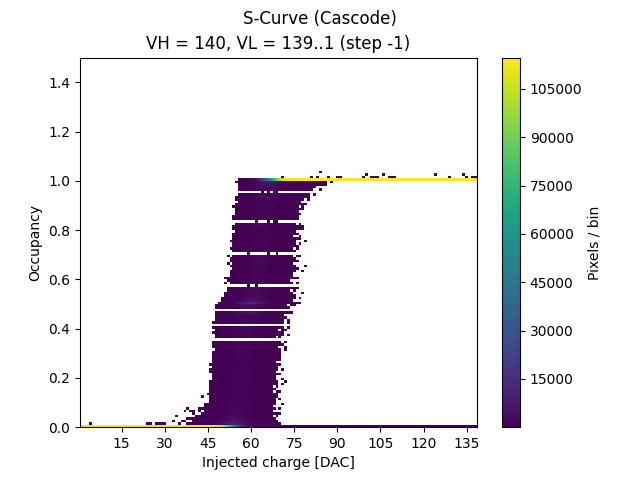
\includegraphics[scale=.5]{all_casc_thscan_140}
\caption{S-curves of all pixels in the \textbf{Cascode} flavor with an injection pulse of 140 DAC.}
\label{fig:casc_scurve140}
\end{figure}

The fit of the threshold distributions instead, are shown in figure \vref{fig:thdist_casc}.

\begin{figure}[h!]
\centering
\subfigure[VH = 140 DAC]
{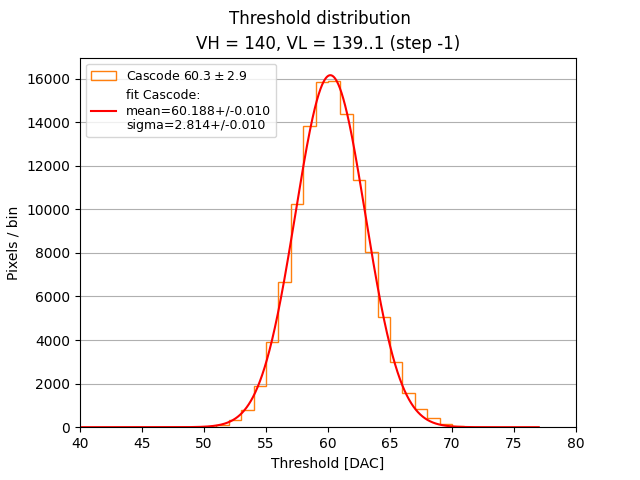
\includegraphics[scale=0.5]{all_casc_thdist_140}}\quad
\subfigure[VH = 200 DAC]
{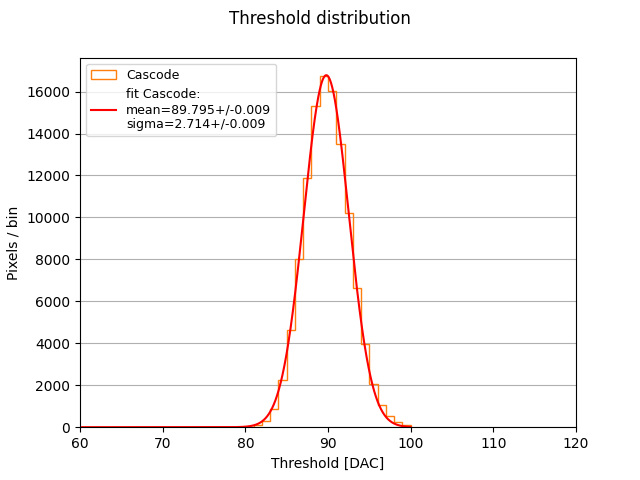
\includegraphics[scale=0.5]{all_casc_thdist_200}}\\
\caption{Threshold distributions of \textbf{Cascode} flavor before and at the maximum saturation, respectively.}
\label{fig:thdist_casc}
\end{figure}


\subsubsection{HV-Cascode FE}

The third flavor is \textbf{HV-Cascode FE} where HV stands for \textbf{High Voltage} and it is formed (counts) of 512 rows and 32 columns for a total number of pixel equal to 16384. Also for these last two flavors, the main chip registers are set with the same values tested and used during the Test Beam (@Desy) (but different from those used for the first two flavors). They are reported in table \vpageref{tab:tb_hv_settings} .

\begin{table}[h!]
\centering
\begin{tabular}{c|c}
Registri & Default Settings (''GOE'') \\
\hline
ITHR & 30 \\
\hline
IBIAS & 60 \\
\hline
VRESET & 100 \\
\hline
ICASN & 8 \\
\hline
VCASP & 40 \\
\hline
VCASC & 228 \\
\hline
IDB & 100 \\
\hline
ITUNE & 53 \\
\hline
VCLIP & 255 \\
\hline
ICOMP & 80 \\
\hline
IDEL & 88 \\
\hline
IRAM & 50 \\
\hline
\end{tabular}
\caption{Settings of the main registers used for the W14R12 chip, for the HV's flavors, during the Test Beam in Desy.}
\label{tab:tb_hv_settings}
\end{table}

As we can see from the plot of the alle S-curves in figure \vref{fig:hvc_scurve_140}, with these choices of values' registers, there were a lot of noisy pixels, but at this stage of measurements they were not masked.
As a matter of fact along the y-axis of this plot is displayed the occupancy and when this values becomes higher than 1, it means that the pixel detects more hits than the injected ones, so it could be identified as ''\textit{noisy pixel}''.
[beacuse it results active regardless of the injection.]


\begin{figure}[h!]
\centering
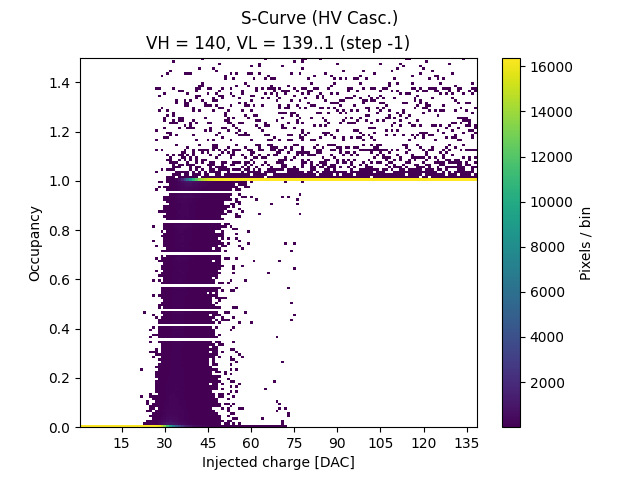
\includegraphics[scale=.5]{all_HVc_thscan_140}
\caption{S-curves of all pixels in \textbf{HV Cascode} flavor with an injection pulse of 140 DAC.}
\label{fig:hvc_scurve_140}
\end{figure}

In figure \vref{fig:thdist_hvc} are shown the fit of the threshold distributions for the two different injections pulse.

\begin{figure}[h!]
\centering
\subfigure[VH = 140 DAC]
{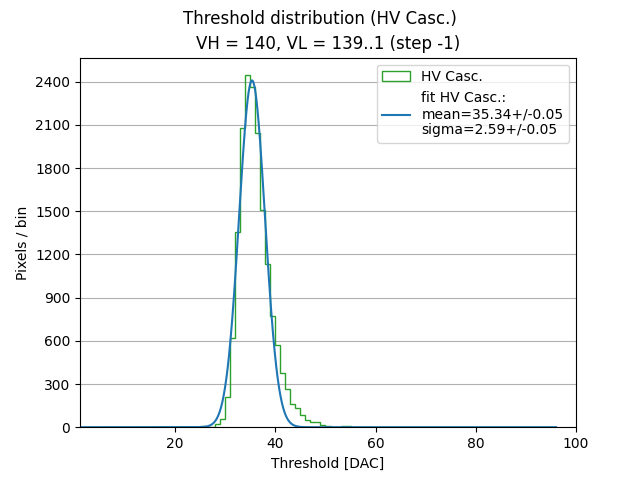
\includegraphics[scale=0.5]{all_HVc_thdist_140}}\quad
\subfigure[VH = 200 DAC]
{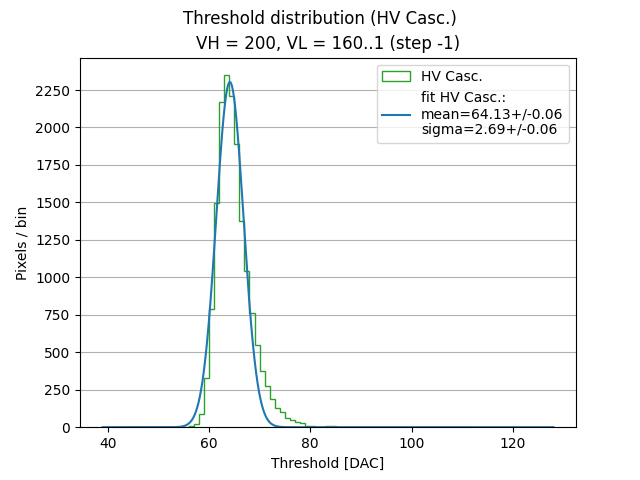
\includegraphics[scale=0.5]{all_HVc_thdist_200}}\\
\caption{Threshold distributions of \textbf{HV Cascode} flavor before and at the maximum saturation, respectively.}
\label{fig:thdist_hvc}
\end{figure}


\subsubsection{HV-Normal FE}

The fourth and last flavor is the \textbf{HV-Normal FE} which consists of 512 rows and 32 columns for a total number of pixel equal to 16.384. The main registers have been set with the values reported in table \vpageref{tab:tb_hv_settings}.
In figure \vref{fig:hv_scurve_140}, the S-curves of all pixel in the flavor. Also here we can see that there were some noisy pixels unmasked.
Moreover, in this final flavor, the last 16 columns were not working and as a matter of fact they had return a peak of threshold near the value 0, which is excluded from the threshold distributions plots.

So actually in this part of the matrix, the real number of pixel studied was the half of the total, such as 8192 pixels.



\begin{figure}[h!]
\centering
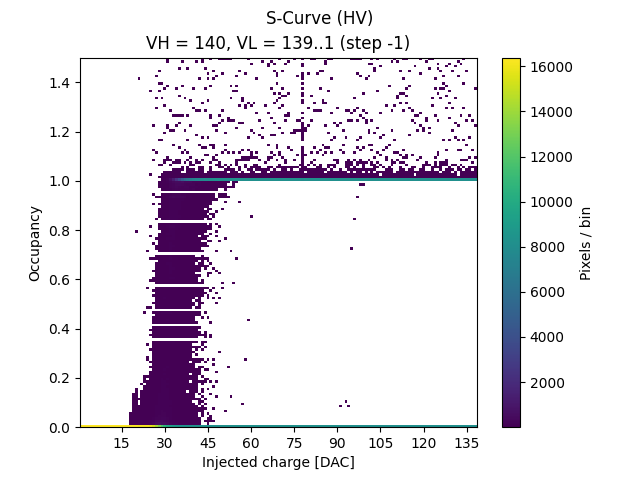
\includegraphics[scale=.5]{all_HV_thscan_140}
\caption{S-curves of all pixels in \textbf{HV Cascode FE} with an injection pulse of 140 DAC.}
\label{fig:hv_scurve_140}
\end{figure}

In figure \vref{fig:thdist_hvc} the fit of the threshold distributions for the two different values of injection height are reported.


\begin{figure}[h!]
\centering
\subfigure[VH = 140 DAC]
{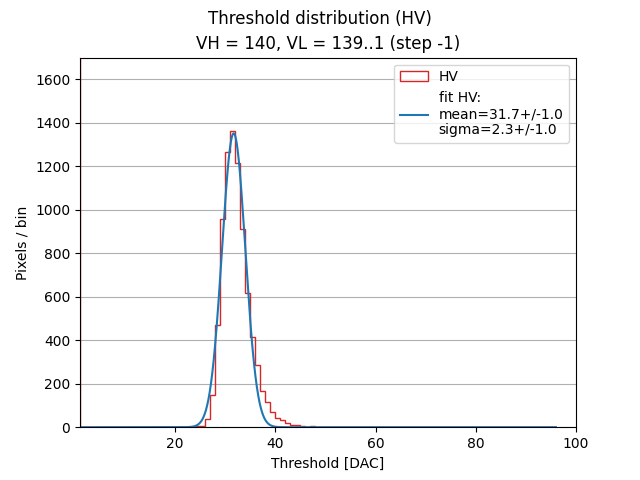
\includegraphics[scale=0.5]{all_HV_thdist_140}}\quad
\subfigure[VH = 200 DAC]
{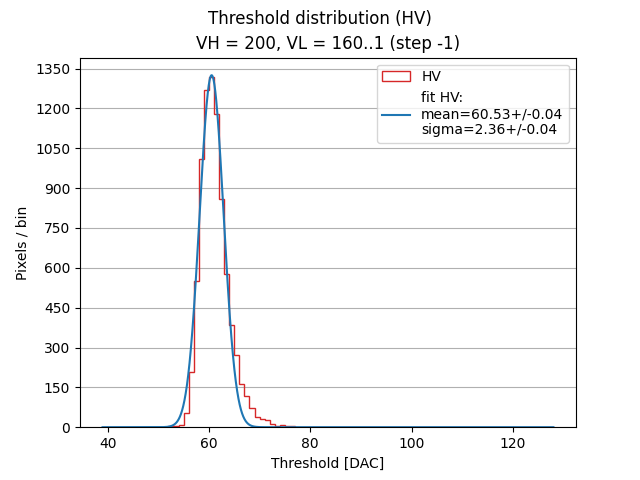
\includegraphics[scale=0.5]{all_HV_thdist_200}}\\
\caption{Threshold distributions of \textbf{HV} flavor before and at the maximum saturation, respectively.}
\label{fig:thdist_hvc}
\end{figure}


\subsection{Noise and Equivalent Noise Charge (ENC)}
%\addcontentsline{toc}{subsection}{Noise and Equivalent Noise Charge (ENC)}

\subsection{Time Over Threshold (TOT) curves and fit}
%\addcontentsline{toc}{subsection}{Curve del Time Over Threshold (TOT) e fit}

A side effect of the injection circuit issue is that the response of the chip can not be characterized in a region of charge that usually corresponds to the emission peaks of the radioactive sources available in the laboratory. 
For this reason, a fit of the ToT obtained at the maximum possible injected charge has been done, in order to extrapolate the most probable value of ToT in the main interesting region of charge.

The function chosen for this purpose is:

\begin{equation}
y(x) = a\cdot x +b -\frac{c}{x-t}
\end{equation}

with \textit{a}, \textit{b}, \textit{c} and \textit{t} free parameters.

Actually we know that the ToT distribution starts to grow near the threshold, so a random parameter could be computed in function of the threshold value estimated from the previous measurements, explained in section (reference).

In particular knowing that y($x_{th}$) must be equal to 0, it can be imposed:

\begin{equation}
0 = a\cdot x_{th} + b - \frac{c}{x_{th}-t}  \hspace{.4cm}	\Rightarrow  \hspace{.4cm}	c = x_{th}^{2}\cdot a + x_{th}\cdot (b-a\cdot t) - t\cdot b
\end{equation}

In this way the number of parameters to fit is reduced.

So the same data collected in the previous measurements of thresholds (for VH=200 DAC unit), have been used to fit the ToT curves of all pixels for each frontend.
In table \vref{tab:th_fe} are reported the value of the threshold considered for each frontend to extrapolate the value of the parameter \textit{c}and the results of the fit for all parameters. In figure \vref{fig:tot_fe} the results obtained for all Normal, Cascode and HVs FE.

\begin{table}[h!]
\centering
\begin{tabular}{c|c|c|c|c}
 & \textbf{Normal} & \textbf{Cascode} & \textbf{HV Cascode} & \textbf{HV} \\
\hline
\textit{threshold [DAC unit]} & 53.62 & 60.19 & 35.34 & 31.70 \\
\textit{a} & & & & \\
\textit{b} & & & & \\
\textit{c} & & & & \\
\textit{t} & & & & \\
\end{tabular}
\caption{Threshold and parameters obtained from the fit of ToT curve for each frontend.}
\label{tab:th_fe}
\end{table}

\begin{figure}[h!]
\centering
\subfigure[\textbf{Normal}]
{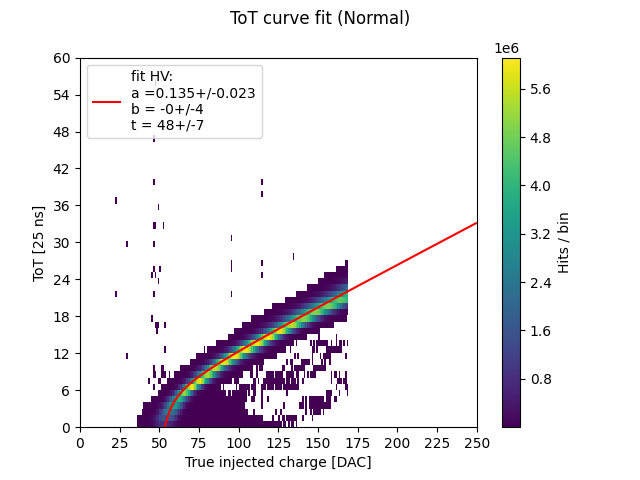
\includegraphics[scale=0.35]{tot_fit_normal(200)}}\quad
\subfigure[\textbf{Cascode}]
{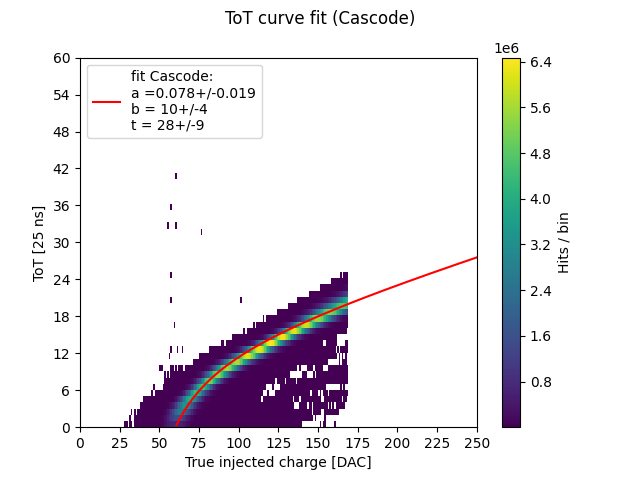
\includegraphics[scale=0.35]{tot_fit_cascode(200)}}\\
\subfigure[\textbf{HV Cascode}]
{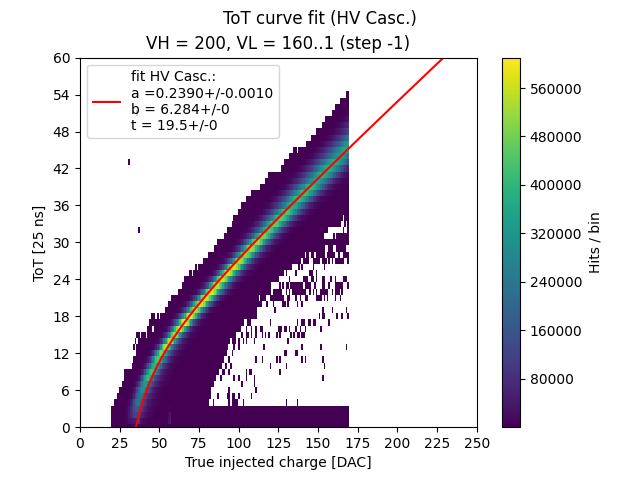
\includegraphics[scale=0.35]{tot_fit_HV_Casc.(200)}}\quad
\subfigure[\textbf{HV}]
{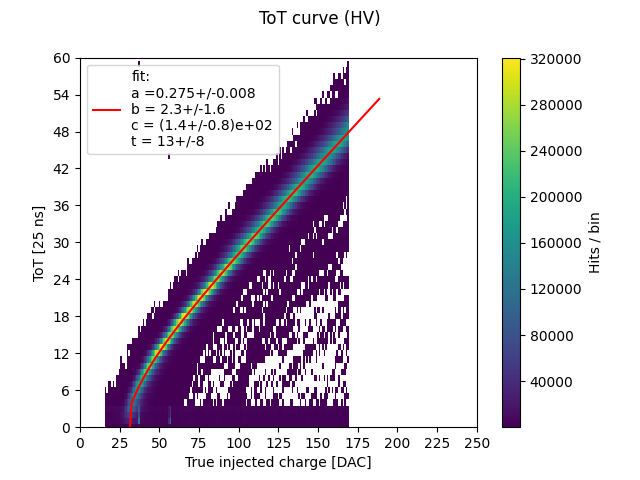
\includegraphics[scale=0.35]{tot_fit_HV(200)}}\\
\caption{ToT curves fit for all frontend.}
\label{fig:tot_fe}
\end{figure}

 












\section{Radioactive sources}
%\addcontentsline{toc}{section}{Caratterizzazione con le sorgenti radioattive}

\subsection{\ch{^{55}Fe}}

\begin{figure}[h!]
\centering
\subfigure[\textbf{Normal}]
{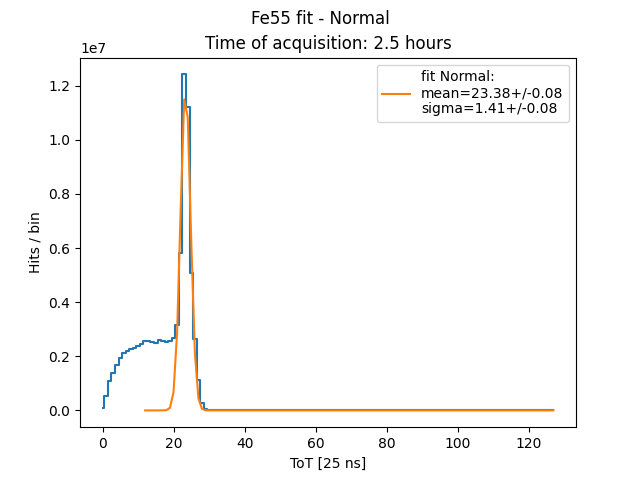
\includegraphics[scale=0.35]{fe55_Normal_peak}}\quad
\subfigure[\textbf{Cascode}]
{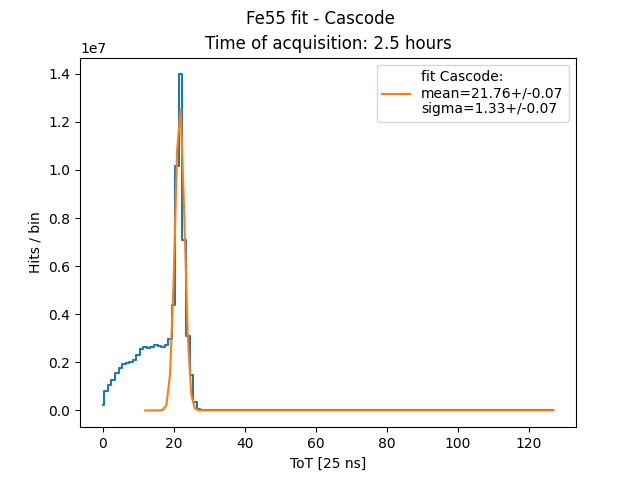
\includegraphics[scale=0.35]{fe55_Cascode_peak}}\\
\subfigure[\textbf{HV Cascode}]
{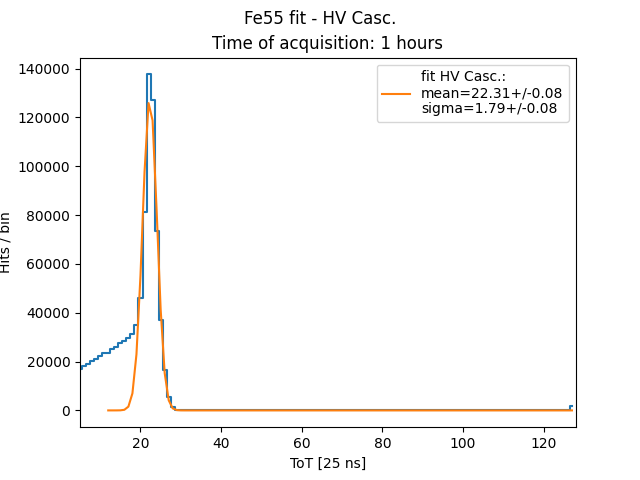
\includegraphics[scale=0.35]{fe_HV Casc._peak}}\quad
\subfigure[\textbf{HV}]
{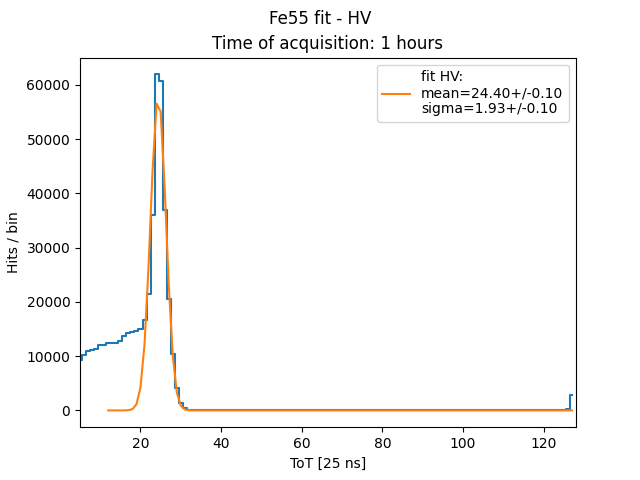
\includegraphics[scale=0.35]{fe_HV_peak}}\\
\caption{\ch{^{55}Fe} pekas for all frontends.}
\label{fig:fe_all}
\end{figure}


CUT ON HVs flavors because of bad columns, many 0 ToT.

\subsection{\ch{^{241}Am}}


\begin{figure}[h!]
\centering
\subfigure[\textbf{Normal}]
{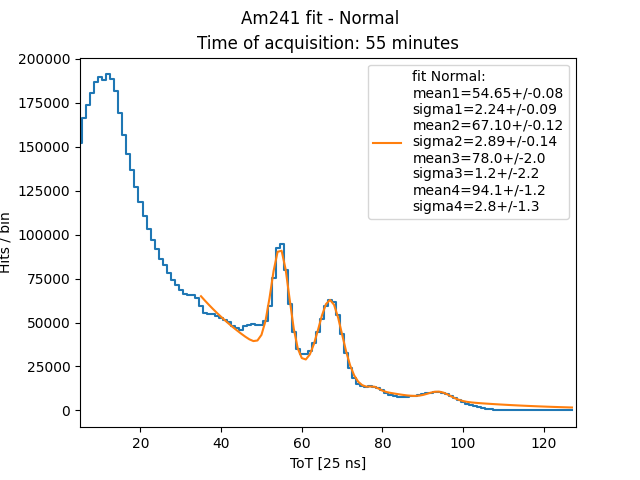
\includegraphics[scale=0.35]{am_Normal_peak}}\quad
\subfigure[\textbf{Cascode}]
{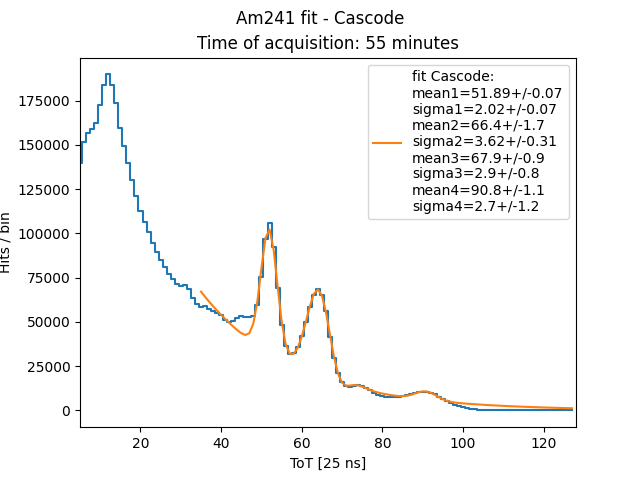
\includegraphics[scale=0.35]{am_Cascode_peak}}\\
\subfigure[\textbf{HV Cascode}]
{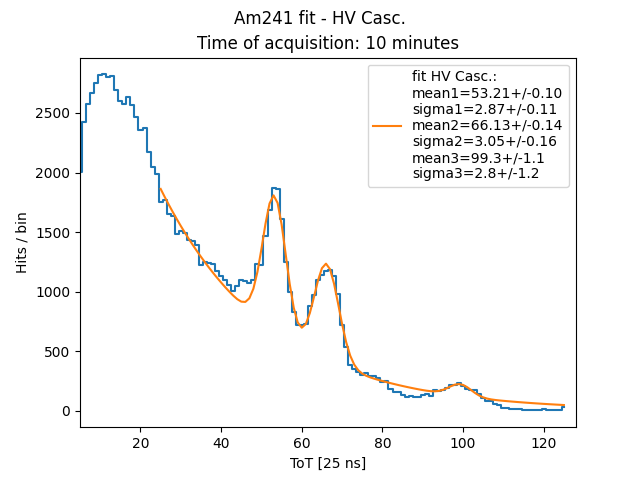
\includegraphics[scale=0.35]{am_HV Casc._peak}}\quad
\subfigure[\textbf{HV}]
{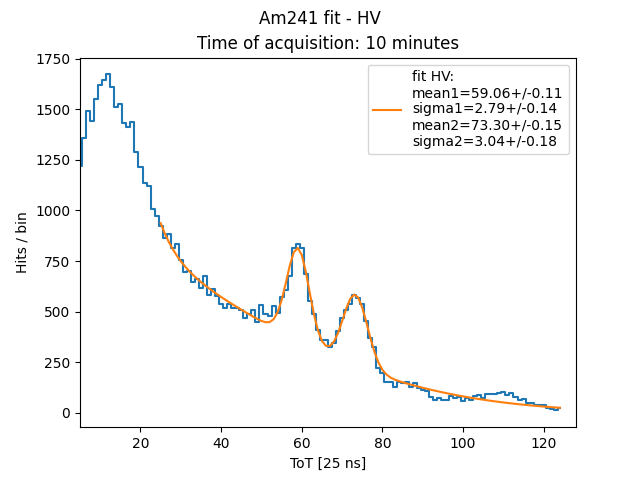
\includegraphics[scale=0.35]{am_HV_peak}}\\
\caption{\ch{^{241}Am} pekas for all frontends.}
\label{fig:fe_all}
\end{figure}



\subsection{\ch{^{109}Cd}}

\begin{figure}[h!]
\centering
\subfigure[\textbf{Normal}]
{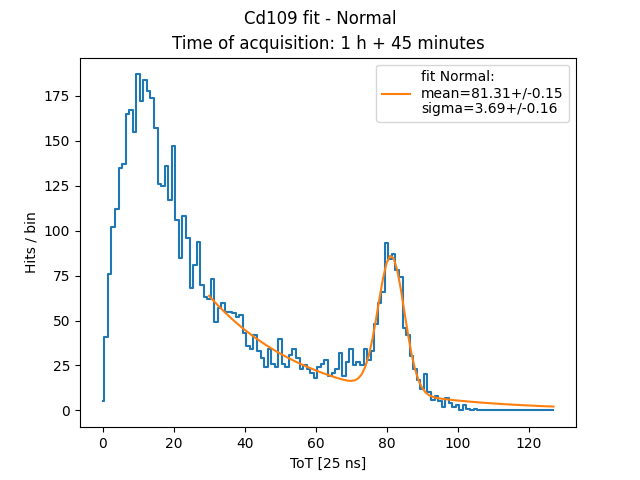
\includegraphics[scale=0.35]{cd109_Normal_peak}}\quad
\subfigure[\textbf{Cascode}]
{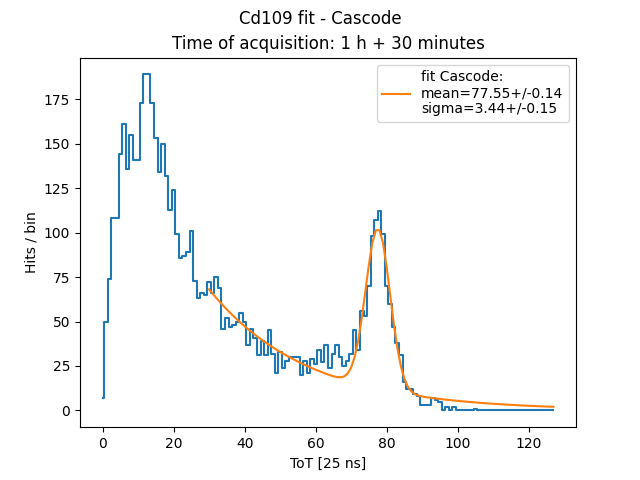
\includegraphics[scale=0.35]{cd109_Cascode_peak}}\\
\subfigure[\textbf{HV Cascode}]
{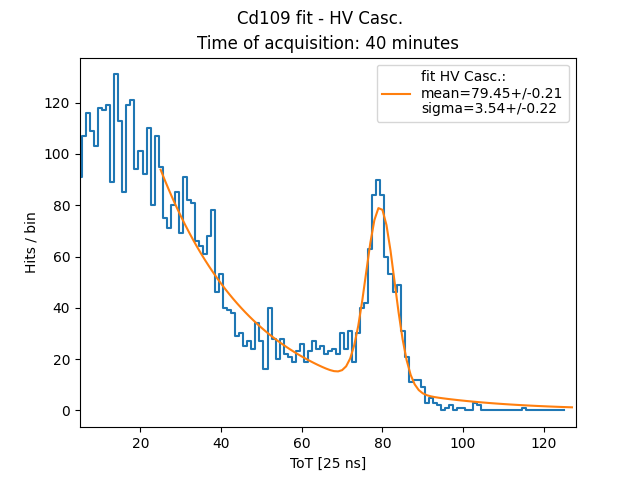
\includegraphics[scale=0.35]{cd109_HV Casc._peak}}\quad
\subfigure[\textbf{HV}]
{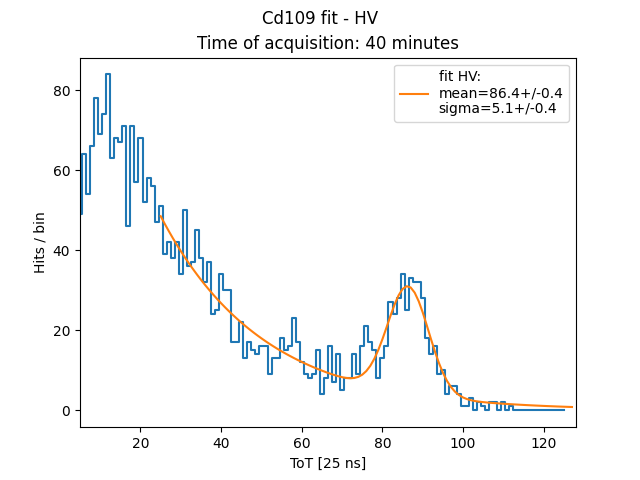
\includegraphics[scale=0.35]{cd109_HV_peak}}\\
\caption{\ch{^{109}Cd} pekas for all frontends.}
\label{fig:fe_all}
\end{figure}

\subsection{\ch{^{190}Sr}}


\subsection{Injection capacitance calibration}
%\addcontentsline{toc}{subsection}{Calibrazione della capacità di iniezione}



%%%%%%%%%%%%%%%%%%%%%%%%%%%%%%
%			COMMENT						
%%%%%%%%%%%%%%%%%%%%%%%%%%%%%%


\begin{comment}
In the prototype under test (the chip W14R12), some problems had come up right from the beginning, for both the analog and digital part of the pixel readout.
Despite its predecessor Tj-Monopix 1, Tj-Monopix 2 is equipped with a circuit which allows the \textit{threshold tuning}. In other words it can adjust every pixel threshold, even if only by few DAC, in order to have a global threshold on the matrix as uniform as possible, or in any case a dispersion as small as possible.
\end{comment}




%%%%%%%%%%%%%%%%%%%%%%%%%%
%			BIBLIOGRPAHY
%%%%%%%%%%%%%%%%%%%%%%%%%%

%1. THESIS MUSTAKAS
